\chapter{Methodology}

- Does the growth reach a steady state? (at t=1200)
- Will the rate of growth reach a steady state or will the number increase as you keep increasing the size of the grid?
- What will happen if the value of M is changed - pick two values on either side of the value given.
- Comment on computational complexity of each method. (note you had been asked to locate common-points which both methods reach)

\section{Cell Movement}

5 marks for definitions of distributions and reasons behind the choice of distribution

The random movement of cells should be modelled using a probability distribution


There are several probability distributions that can be classified as discrete or continuous, we will analyse uniform, bernoulli and beta.

The uniform distribution is usually regarded as a continuous distribution but can also be used to model discrete variables. 

Area under the graph is one

\[ f(x) =\begin{cases}a & \text{if } x = 1\\b & \text{if } x = 0\end{cases}\]

\[ f(x) =\begin{cases}1 & \text{for } 0  \leq x  \leq  1\\0 & \text{otherwise}\end{cases}\]

Uniform distribution
Definition of distributions
Uniform distributions
Bernoulli Distribution

Bias introduced with different distributions


When all directions are equally probable a uniform distribution could be used.

If a Bernoulli distribution was selected, it would introduce a bias to the direction of movement
This could be desired in a complex model where factors such as surface tension affect the direction of movement


% how random numbers are actually generated in rust



% complexity of the different movements
%  all o^n but increase the multiplier of n







Movement directions

'Complexity of direction methods'

\clearpage

\begin{figure}[ht]
    \centering
    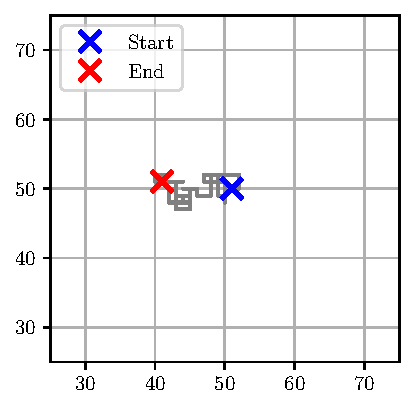
\includegraphics[width=5cm]{task1-1}
    \caption[Square cell movement plot]{Square cell movement plot}
    \label{fig:task1-1}
\end{figure}

\begin{figure}[ht]
    \centering
    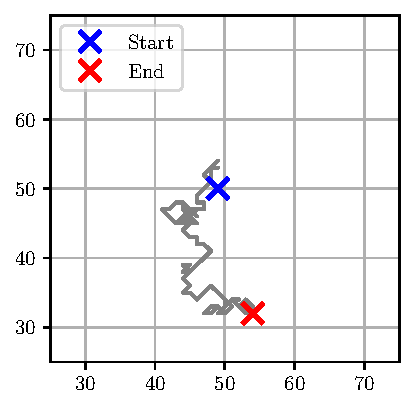
\includegraphics[width=5cm]{task1-2}
    \caption[Diagonal cell movement plot]{Diagonal cell movement plot}
    \label{fig:task1-2}
\end{figure}

\begin{figure}[ht]
    \centering
    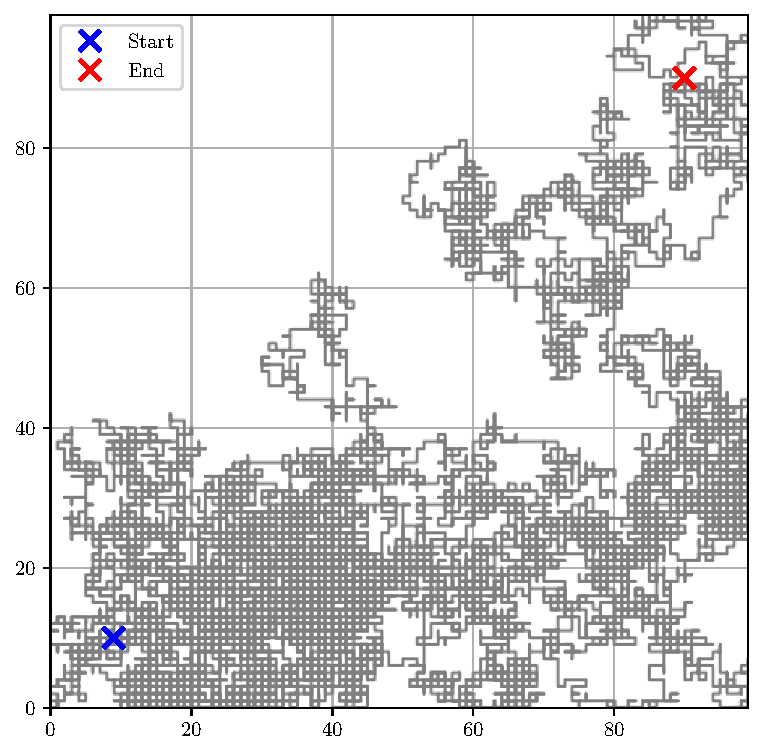
\includegraphics[width=10cm]{task1-1-fill}
    \caption[Square cell movement plot with fill]{Square cell movement plot with fill}
    \label{fig:task1-1-fill}
\end{figure}

\begin{figure}[ht]
    \centering
    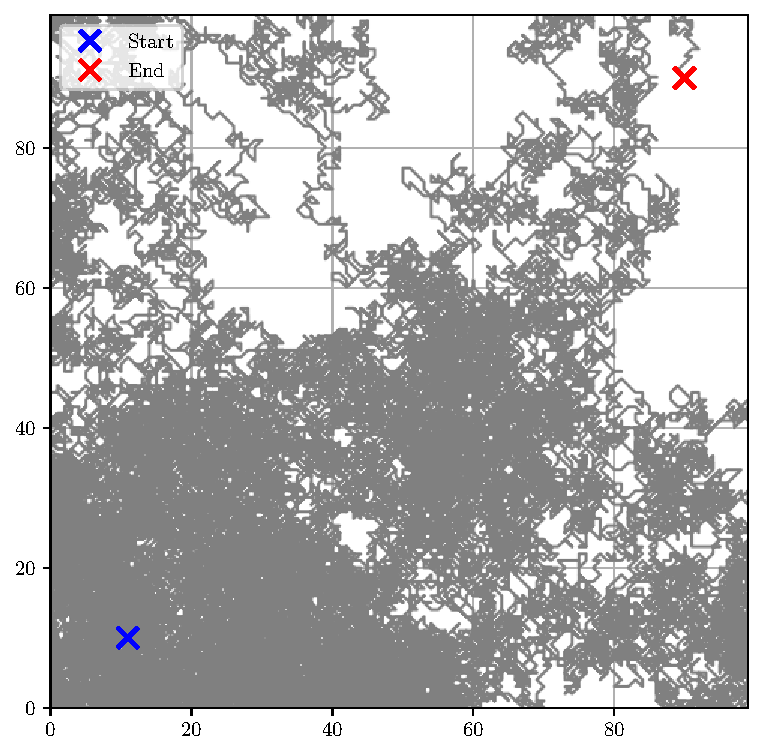
\includegraphics[width=10cm]{task1-2-fill}
    \caption[Diagonal cell movement plot with fill]{Diagonal cell movement plot with fill}
    \label{fig:task1-2-fill}
\end{figure}

\clearpage

\begin{figure}[ht]
    \centering
    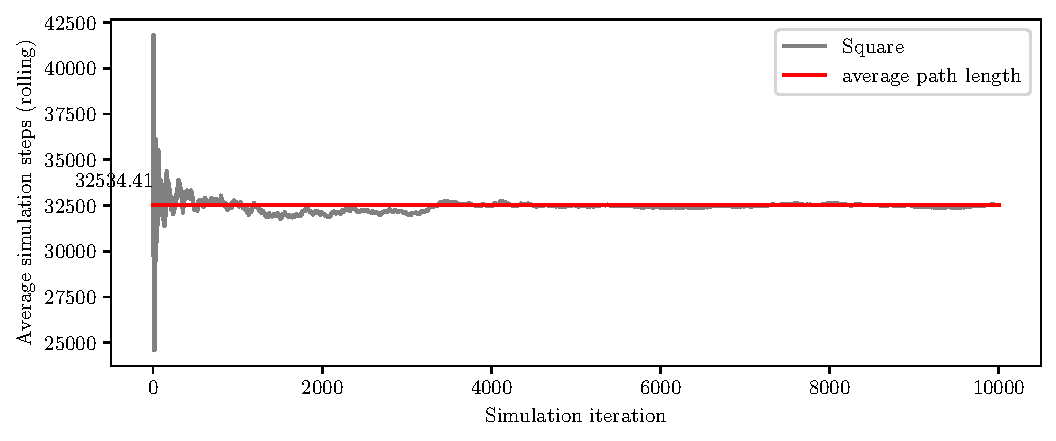
\includegraphics[width=14cm]{task1-compare-square-roll}
    \caption[Square cell simulation steps]{Square cell simulation steps}
    \label{fig:task1-compare-square-roll}
\end{figure}

\begin{figure}[ht]
    \centering
    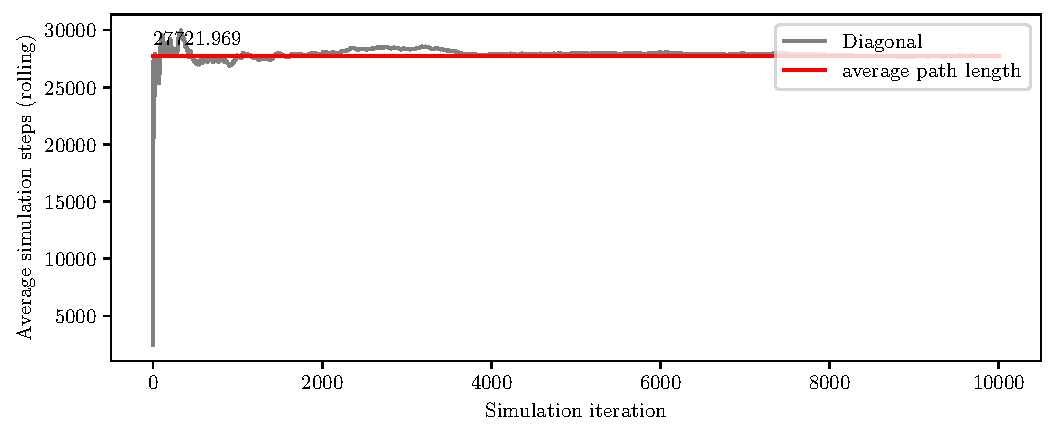
\includegraphics[width=14cm]{task1-compare-diagonal-roll}
    \caption[Diagonal cell simulation steps]{Diagonal cell simulation steps}
    \label{fig:task1-compare-diagonal-roll}
\end{figure}

\clearpage

\begin{figure}[ht]
    \centering
    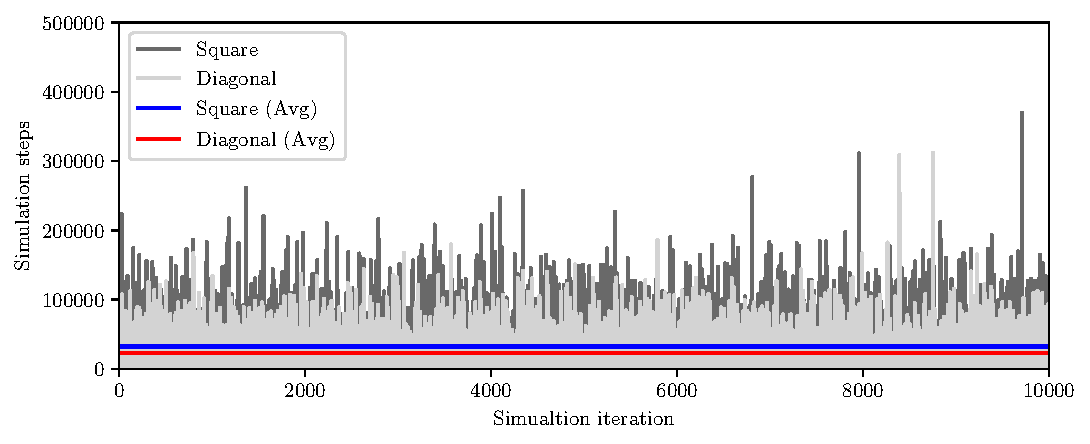
\includegraphics[width=14cm]{task1-compare-single}
    \caption[Comparison of square and diagonal simulation steps]{Comparison of square and diagonal simulation steps}
    \label{fig:task1-compare-single}
\end{figure}

\begin{figure}[ht]
    \centering
    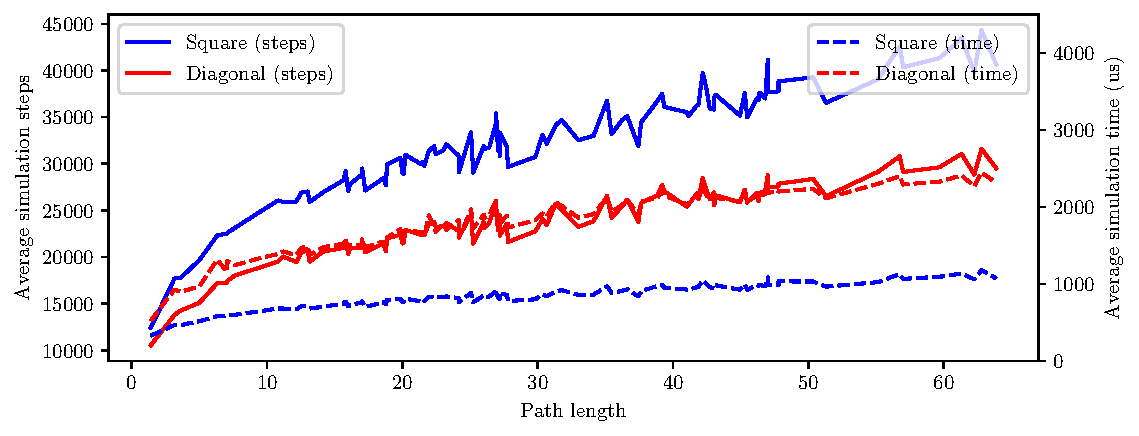
\includegraphics[width=14cm]{task1-compare}
    \caption[Comparison of multiple square and diagonal simulation steps]{Comparison of multiple square and diagonal simulation steps}
    \label{fig:task1-compare}
\end{figure}

\clearpage

\begin{figure}[ht]
    \centering
    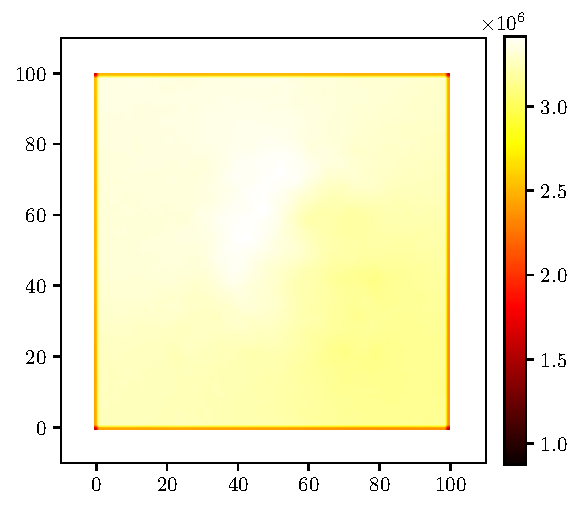
\includegraphics[width=7cm]{task1-visited-square}
    \caption[Visited cells in square simulation heatmap]{Visited cells in square simulation heatmap}
    \label{fig:task1-visited-square}
\end{figure}

\begin{figure}[ht]
    \centering
    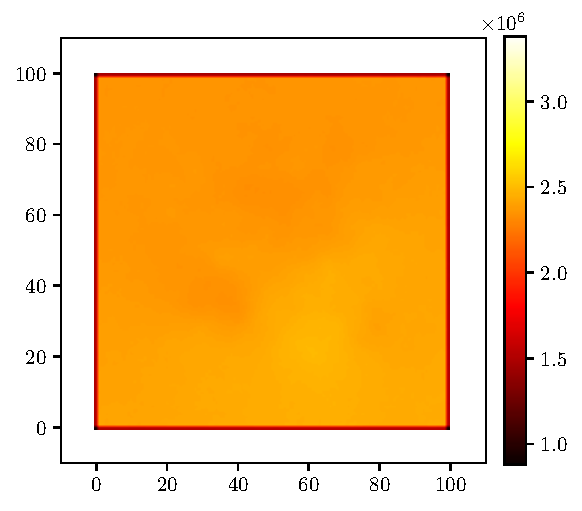
\includegraphics[width=7cm]{task1-visited-diagonal}
    \caption[Visited cells in diagonal simulation heatmap]{Visited cells in diagonal simulation heatmap}
    \label{fig:task1-visited-diagonal}
\end{figure}

\begin{figure}[ht]
    \centering
    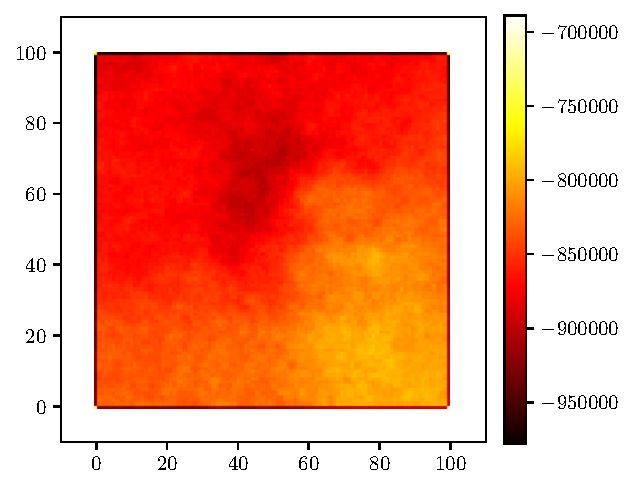
\includegraphics[width=7cm]{task1-visited-diff}
    \caption[Difference in visited cells between square and diagonal simulation heatmap]{Difference in visited cells between square and diagonal simulation heatmap}
    \label{fig:task1-visited-diff}
\end{figure}

\clearpage

\section{Cell Growth}
10 marks for basic simulation, 5 marks for showing time to reach final time 
You can also use analytical methods to do the same

5 marks for the part where you suggest what happens when the value of M changes, and why this is important
\[ \frac{dN}{dt}  = kNln\left(\frac{M}{n} \right) \]

\clearpage

\begin{figure}[ht]
    \centering
    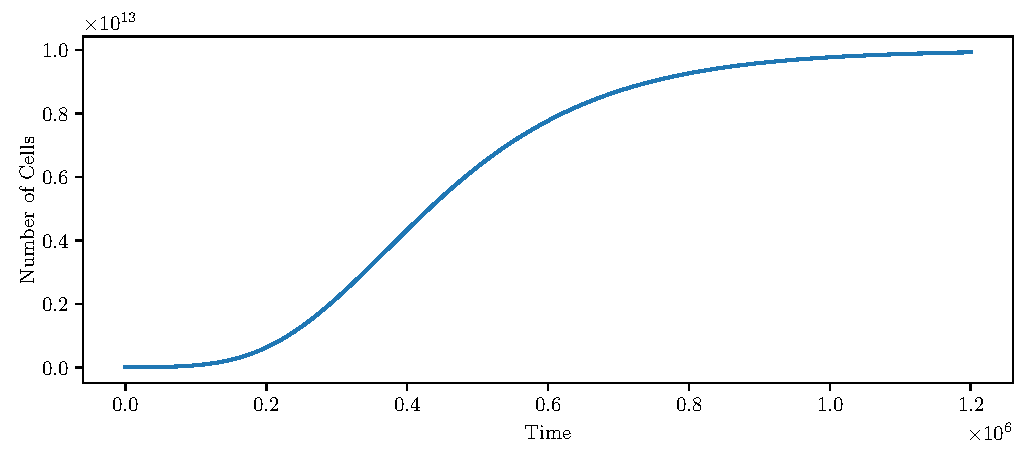
\includegraphics[width=14cm]{task2-1}
    \caption[Cell growth simulation]{Cell growth simulation}
    \label{fig:task2-1}
\end{figure}

\begin{figure}[ht]
    \centering
    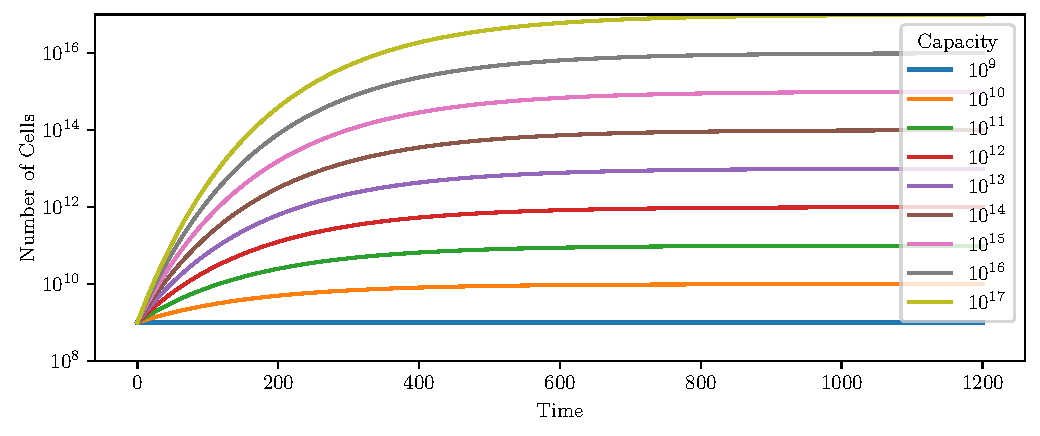
\includegraphics[width=14cm]{task2-1-m}
    \caption[Cell growth simulation with different capacity values]{Cell growth simulation with different capacity values}
    \label{fig:task2-1-m}
\end{figure}

\clearpage

\begin{figure}[ht]
    \centering
    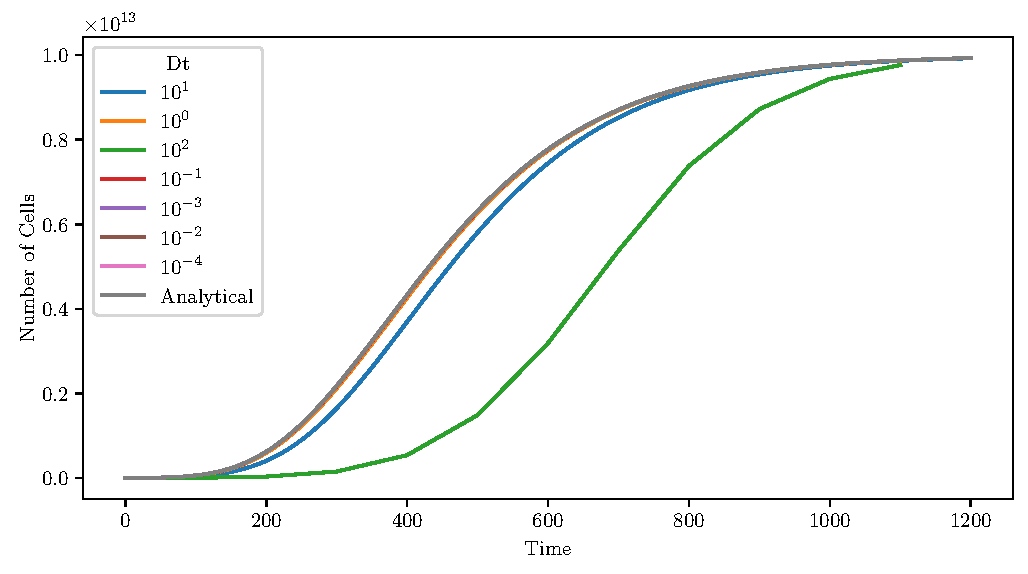
\includegraphics[width=14cm]{task2-1-h}
    \caption[Cell growth simulation with different dt values]{Cell growth simulation with different dt values}
    \label{fig:task2-1-h}
\end{figure}

\begin{figure}[ht]
    \centering
    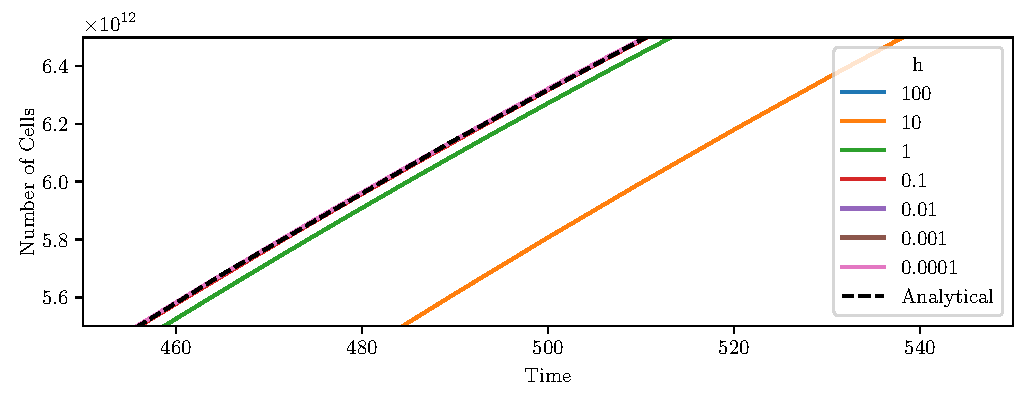
\includegraphics[width=14cm]{task2-1-h-zoom}
    \caption[Cell growth simulation with different dt values (zoomed)]{Cell growth simulation with different dt values (zoomed)}
    \label{fig:task2-1-h-zoom}
\end{figure}

\clearpage

\begin{figure}[ht]
    \centering
    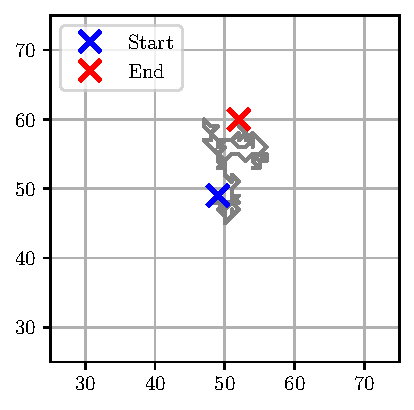
\includegraphics[width=5cm]{task2-2}
    \caption[Cell growth simulation with diagonal movement]{Cell growth simulation with diagonal movement}
    \label{fig:task2-2}
\end{figure}

\begin{figure}[ht]
    \centering
    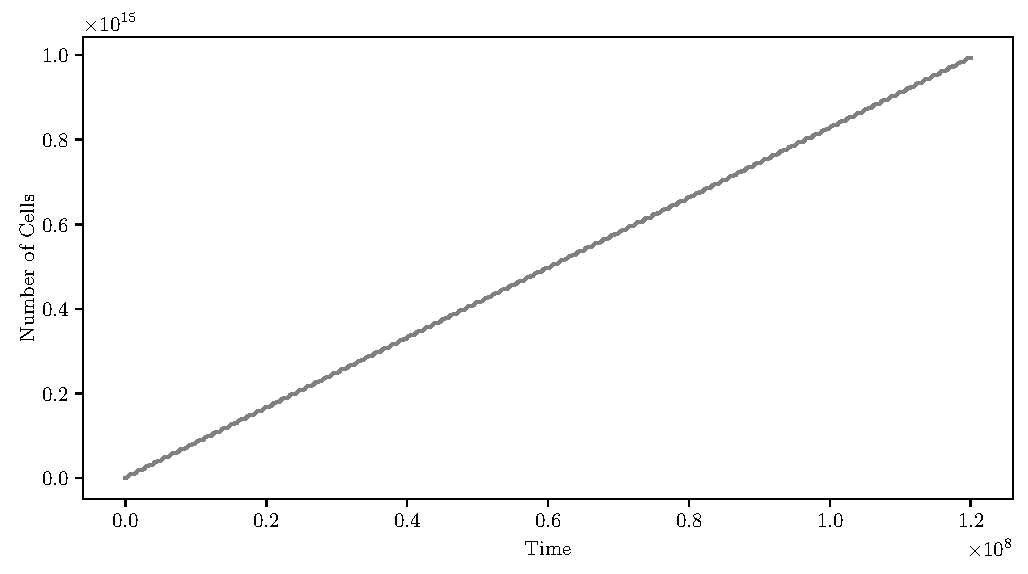
\includegraphics[width=14cm]{task2-2-total}
    \caption[Cell growth simulation with diagonal movement (total cells)]{Cell growth simulation with diagonal movement (total cells)}
    \label{fig:task2-2-total}
\end{figure}

\begin{figure}[ht]
    \centering
    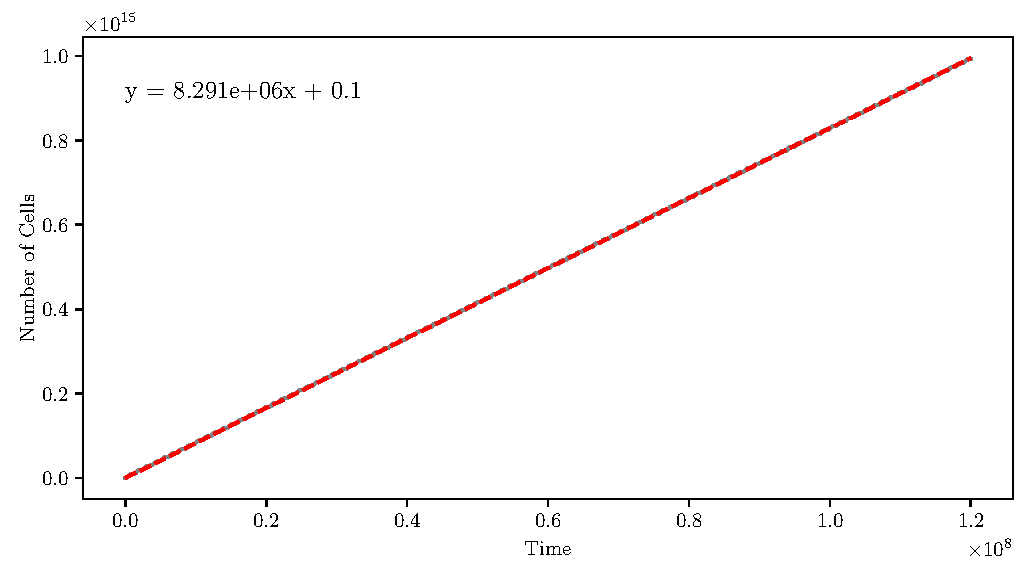
\includegraphics[width=14cm]{task2-2-total-linear}
    \caption[Cell growth simulation with diagonal movement (total cells) linear estimation]{Cell growth simulation with diagonal movement (total cells) linear estimation}
    \label{fig:task2-2-total-linear}
\end{figure}
